\documentclass[sotsuron]{jcsie}
\usepackage[dvipdfmx]{graphicx}
\usepackage{float}
\usepackage{listings}

\lstset{
  basicstyle={\ttfamily},
  identifierstyle={\small},
  commentstyle={\smallitshape},
  keywordstyle={\small\bfseries},
  ndkeywordstyle={\small},
  stringstyle={\small\ttfamily},
  frame={tb},
  breaklines=true,
  columns=[l]{fullflexible},
  numbers=left,
  xrightmargin=0zw,
  xleftmargin=3zw,
  numberstyle={\scriptsize},
  stepnumber=1,
  numbersep=1zw,
  lineskip=-0.5ex
}

\title{ライブストリーミングに対応した分散ハッシュテーブルの検討}
\etitle{Distributed hash table for live streaming}
\author{沈 嘉秋}
\eauthor{Yoshiaki Shin}
\id{T18I917F}
\keywords{P2P, 分散ハッシュテーブル}
\ekeywords{P2P, distributed hash table}

\begin{document}
\maketitle
\emaketitle
\pagenumbering{roman}
\begin{abstract}    
	分散ハッシュテーブルはファイル共有サービス等に応用され、
	すでに普及している一方で、
	近年はブロックチェーンの関連技術としても注目を集めている。
	分散ハッシュテーブルの中でもKademlia
	はその実装の容易さとノードの出入りに対する耐性の強さから
	実用的なサービスへの応用が可能であり、
	多くのサービスで採用されている。
	近年、ライブストリーミングサービスの需要が高まっている
	一方で配信プラットフォームの事業者への依存が強く
	サービス利用者の立場は弱いものとなっている。
	そこで本論文では
	分散的なライブストリーミングサービスの基盤となる
	システムをKademliaを元に実装し、その評価を行った。
	Kademlia上で単純にライブストリーミングの実装を行う場合、
	非効率的な通信が発生するが、本論文の手法では、
	Kademliaネットワークを更に構造化することで
	非効率的な通信を削減することが可能となった。
	結果、分散的なライブストリーミングサービスの実装への
	足がかりを作ることが出来た。
\end{abstract}
\begin{eabstract}
	While distributed hash tables have been widely used in file-sharing services,
	they have recently attracted attention as a blockchain-related technology. 
	Among the distributed hash tables, 
	Kademlia can be applied to practical services because of 
	its ease of implementation and resistance to incoming and outgoing nodes, 
	and it is used in many services. 
	In recent years, while the demand for live streaming services has been 
	increasing, there has been a strong dependence on providers of distribution 
	platforms, and the position of service users has become weak. 
	In this paper, we evaluate a system based on Kademlia, 
	which is the basis of distributed live streaming services. 
	When live streaming is simply implemented on Kademlia, 
	inefficient communication occurs, but this paper can reduce inefficient 
	communication by further structuring the Kademlia network. 
	As a result, we were able to create a foothold for implementing a 
	distributed live streaming service.
\end{eabstract}
\setcounter{tocdepth}{2}
\tableofcontents
\pagenumbering{arabic}

% ---------------------------------------------------------------------

\chapter{序論}
\section{背景}
近年、P2Pネットワーク技術がブロックチェーンなどによって再び注目を集めている。
最近ではブロックチェーン流行以前に研究されていた
P2Pネットワーク技術を利用した分散型ファイル共有サービスと
組み合わせて開発されたサービスも登場している。
\cite{BitTorre1:online}
分散型ファイル共有サービスは分散ハッシュテーブルという技術を用いて
実装されることがあり、分散型ファイル共有サービスの中でも
利用者の特に多いBitTorrent\cite{BitTorre59:online}
ではKademlia\cite{maymounkov2002kademlia}\cite{高野祐輝2010nat}
という分散ハッシュテーブルを
用いて開発されている。
分散型ファイル共有サービスはこれまで、膨大なサーバリソースを持つ
大企業などでなければ実現できなかった、大規模かつ、高速な
ファイル共有を実現した。

近年の家庭用ネットワークやモバイルネットワークの環境改善に伴い
Youtube Live\footnote{https://www.youtube.com/live} や 
Twitch\footnote{https://www.twitch.tv} 
といった高いスループットが要求される動画ライブストリーミングサービス
が急速に普及してきている。
しかし、これらのサービスは膨大なサーバリソースを持つ大企業
や大企業の提供するクラウド環境を利用するなどしなければ実現できず、
プラットフォーム事業者やクラウド事業者への依存が強く、
サービス利用者の立場は弱いものとなっており不健全な状態にある。

\section{目的}
分散ハッシュテーブルの中でもKademliaはその実装の容易さと
churn耐性\footnote{ノードの出入りに対する耐性の強さ}
を持つことから実用的なサービスへの応用が可能であるが、
その一方でKademlia上で単純にライブストリーミングの実装を行う場合、
非効率的な通信が発生する。

そこで本論文では、分散型の動画ライブストリーミングサービスの基盤
となるシステムを、Kademliaをベースに実装する。
成果物がWebブラウザとNode.jsで動作するライブラリとなるように開発を行う。

成果物ができるだけ多くのプラットフォームで動作するようにするために
P2P通信箇所にWebRTC \cite{WebRTCHo80:online}
を用いる。WebRTCはWebブラウザなどといったフロントエンド
環境とサーバーサイド環境の両方に対応した低遅延通信のための規格である。
またWebRTCは近年では、スマートフォンやパーソナルコンピュータに搭載されている
Webブラウザで動作する唯一のP2P通信規格でもある。

完成したライブラリを用いたベンチマークプログラムと
一般的なKademliaを用いたベンチマークプログラムをNode.js上で実行し
その性能や性質の比較を行い有用性などの検証を行う。
完成したライブラリを用いてWebブラウザ上で動作する
分散ライブ動画配信アプリのサンプルを開発し動作確認を行う。

\section{本論文の構成}
本論文ではTypeScriptというプログラム言語を用いて研究を行っている。
そのため、本文中に登場するコードサンプルはすべてTypeScriptによるものである。

% ---------------------------------------------------------------------

\chapter{関連研究}
\section{分散ハッシュテーブル}
分散ハッシュテーブルとは、分散型のkey-valueストアを実現する手法であり、
あるデータとそのハッシュ値をペアとしたハッシュテーブルを
P2Pネットワーク上で複数のノードによって分散的に実装する技術である。
複数のノードにデータを分散配置を行うため適切な構造化を行う必要がある。
構造化には様々な手法が存在し、
ChordやKademliaといったさまざまな実装が存在する。
分散ハッシュテーブルの実装の優劣はデータの探索効率、
Churn耐性、実装の容易さなどによって付けられる。

\section{Kademlia}
Kademliaとは分散ハッシュテーブルの一種である。
高いChurn耐性を持つため、実用的なP2Pアプリケーションにて多く利用されている。
Kademliaはノード数Nのシステムにおいてデータを探索する際に
$O(\log(n))$ 回ノードへの通信を行う。

\subsection{採用例}
Kademliaは高いChurn耐性を持ちながら、実装も容易であるため、
多くの分散型のサービスで利用されている。
ここでは、Kademliaを利用している有名なサービスを幾つか紹介する。
サービスの紹介を表\ref{table:kademlia-services}に示す。
\begin{table}[H]
	\caption{Kademliaを利用したサービス}	
	\centering
	\label{table:kademlia-services}
	\begin{tabular}{|l|l|}
		\hline
		サービス名 & 使用箇所 \\ 
		\hline
		Torrent         &              
		\begin{tabular}{l}
		magnetURLという機能を用いてファイルをダウンロードする際に\\
		目的のファイルを持っているノードを探索するのにKademliaを用いている。\\
		Torrentはアクティブユーザと転送量という点で見ると\\
		世界で最も成功したP2Pのシステムであり、\\
		そのシステムにKademliaはおおいに貢献していると言える。\\
	\end{tabular}\\ \hline
	Ethereum &
	\begin{tabular}{l}
		Node Discovery Protocol v4 というノードの探索プロトコルに用いられている. 
	\end{tabular}\\ \hline
	IPFS     &
	\begin{tabular}{l}
		IPFSとは複数のノードが協調して一つの大きなストレージ                         \\
		またはHTTPの置き換えとして機能することを目的としているシステムある。 \\
		IPFSはKademliaをベースとして開発されている                                            \\
	\end{tabular}\\ \hline
	\end{tabular}
\end{table}

\subsection{Kademliaのアルゴリズム}
\subsubsection{ノードIDとキー}
Kademliaでは個々のノードに固有のノードIDが割り振られており、
このIDを元にルーティングを行う。このノードIDは160bitと定義されている。
ノードIDの決定方法は、ランダムな値にsha1というハッシュ関数を適用し、
160bitの値を取り出すのが一般的である。
また、ハッシュテーブルに保存するバリューと対になるキーも
160bitと定義されている。
\subsubsection{経路表}
分散ハッシュテーブルのアルゴリズムによって
ノードを管理する経路表の形は様々である。
例えば、Chordという分散ハッシュテーブルの場合は環状の経路表を持っている。
Kademliaはk-bucketsという160個のk-bucketからなる経路表を持っている。
一つのk-bucketにはK個(たいていの実装例では20個)のノードが登録でき、
自身のノードとの距離に応じたk-bucketにそれぞれのノードが登録されていく。
ノード間の距離は2進数のノードID同士をXORで掛け合わした結果を
10進数に戻した値を用いる。
\subsubsection{プロトコル}
Kademliaには4種類の通信問い合わせがある。名称と内容についてまとめる。
\begin{table}[H]
	\begin{tabular}{|l|l|}
		\hline
		名称 &   
		内容 \\ 
		\hline
		PING   &   
		\begin{tabular}{l}
		対象のノードがオンラインかどうかを問い合わせる。
	\end{tabular}\\ 
	\hline
	STORE &
	\begin{tabular}{l}
		対象ノードにkey,valueの組を保持させる。                            \\
		保持させる際のルールは、                                              \\
		自身のk-bucketsから最もkeyにxorの距離が近いノードを選択し、 \\
		そのノードにkey,valueを与える。                                        \\
		受け取ったノードは更に自身のk-bucketsから受け取ったkeyに    \\
		最も近いノードを選択し、                                              \\
		key,valueを与える。この動作を何度も繰り返す。                   \\
		最終的にはネットワーク上で最もkeyに距離が近いノードが    \\
		目的のkey,valueを持つ。                                                    
	\end{tabular}\\
	\hline
	FIND\_NODE &
	\begin{tabular}{l}
		自身のk-bucketsのうち最もkeyにxor距離の近いノードに                   \\
		自身のノードIDと距離が近い上位K個のノードの情報を送らせる。 
	\end{tabular}\\
	\hline
	FIND\_VALUE &
	\begin{tabular}{l}
		自身のk-bucketsのうち最もkeyにxor距離の近いノードに                      \\
		keyと対応するvalueを持っているか問い合わせる。                          \\
		持っている場合はそのvalueを、                                                  \\
		持っていない場合は問い合わせられたノード自身のk-bucketsのうち、 \\
		keyに最も近いノードの情報を返す。                                           
	\end{tabular}\\
	\hline
	\end{tabular}
\end{table}
\subsubsection{ノードの管理}
KademliaのChurn耐性の高さはこのノードの管理方法にある。
Kademliaのノード管理は上記の4つのプロトコルの通信を行うついでに行われる。
そのため、ノードの離脱の際の処理が必要なく、
Churnを考慮することなくネットワークを維持することができる。
\subsubsection{経路表の更新}
ノードは4つのプロトコルのいずれかのメッセージを受け取った際に
送信元が該当するk-bucketの中にあった場合そのノードをk-bucketの末尾に移す。
送信元が該当するk-bucketの中に存在しないせず、k-bucketがすでに満杯な場合、
そのk-bucket中の先頭のノードがオンラインかどうかをPINGで確認する。
オンラインなら先頭のノードを残し、
そうでなければ送信元の新しいノードをk-bucketに追加する。
こうすることで長時間オンラインになっているノードが優先的にk-bucketに残るため、
ネットワークの安定性が増す。
\subsubsection{ノードの新規参加}
新規参加するノードは、
まず接続先のノードに対して自身のノードIDをkeyとしてFIND\_NODEを行う。
問い合わせを受けたノードは送信元のkeyに近い最大K個のノードの情報を
送信元にSTOREする。
そうすることで、新規参加するノードはまず最大K個のノードに接続される。
このあと、さらに自身のk-bucketsのうち最も自身のノードIDに
xor距離が近いノードに対し自身のノードIDをkeyとしたFIND\_NODEを
繰り返すことで接続先のノードを増やすことができる。
\subsubsection{ノードの離脱}
何もしない

\section{WebRTC}
WebRTCとはWorld Wide Web Consortium(W3C)\footnote{https://www.w3.org/}
が提唱するリアルタイムコミュニケーション用のAPIの定義で,プラグイ
ン無しでウェブブラウザ間のボイスチャット,ビデオチャット,ファイル共有
ができる.ブラウザでリアルタイムなコミュニケーションを可能にする
WebRTCはGoogleによってオープンソース化されており,現在は,W3Cによっ
てブラウザ対応APIの標準化が進められているWebRTCはブラウザ向けのAPIと
して誕生したが,現在では,AndroidやiOSといったネイティブ環境で実装する
ためのライブラリが公開されている.WebRTCにはNAT越えを実現するために
Interactive Connectivity Establishment (ICE)\cite{rosenberg2010interactive}
という仕組みを採用している。
\subsection{NAT越え}
NAT(Network Address Translation)とは,
インターネットプロトコルによって構築されたコンピュータネットワークにおいて,
パケットヘッダに含まれるIPアドレスを,別のIPアドレスに変換する技術である.
プライベートネットワーク環境下でプライベートIPアドレスを持つホストから,
グローバルIPアドレスを持つゲートウェイを通して,
インターネットにアクセスする際に,プライベートIPアドレスを
グローバルIPアドレスに変換するために利用されることが多い.
モバイルネットワークにおいてはキャリアグレードNATが用いられている.
そのため,スマートフォン間でP2P通信を行うためには,
NAT越えを行う必要がある.
本研究ではWebRTCを用いてNAT越えを行う.
WebRTCではICEの情報をやり取りすることで,NAT越えを行っている.
ICEとは通信可能性のある通信経路に関する情報を示し,
文字列で表現される.次のような複数の経路を候補とする.\\\\
・P2Pによる直接通信\\
・STUNによる,NAT通過のためのポートマッピング\\
・TURNによる,リレーサーバーを介した中継通信\\

STUN\cite{wing2008session}とは,
音声,映像,文章などの双方向リアルタイムIP通信を行うアプリケーションにおいて,
NAT越えの方法の1つとして使われる標準化されたインターネットプロトコルである.
STUNプロトコルは,アプリケーションがNATの存在と種類を発見し,
リモートホストへのUDP接続に
NATが割り当てたグローバルIPアドレスとポート番号とを得ることを許す.
STUNプロトコルが動作するには,インターネット上にSTUNサーバが存在する必要がある.

TURN\cite{matthews2010traversal}とは,
マルチメディアアプリケーションがNATやファイアウォールを
超えて通信することを補助するためのインターネットプロトコルである.
TURNが一番役立つのは,TCP, UDPを使って
対象型NAT装置により隠蔽(マスカレード)されたプライベートネットワークに
接続されたクライアントを利用する場合である.

本研究ではGoogleが無料公開しているSTUNを用いている.TURNは自ら
TURN用のサーバを構築する必要があるうえ,全ての通信はTURNサーバを経由
するため,TURN上でのデータの転送量が非常に多くなるので本研究ではTURN
サーバを利用していない.
\subsection{シグナリング}
WebRTCでは,SDPとICE Candidateの二つの情報を端末間で交換することによって
P2P通信が開始される.このSDP等を交換する作業をシグナリングと言う.
シグナリングを行うためにはSDP等を交換する必要がある.
シグナリングにはTrickle IceとVanilla Iceの2つの方法がある。
本研究ではVanilla Iceというシグナリング手法を用いる.
Vanilla Iceは,実装が容易である,
シグナリングサーバとの通信回数が少ないというメリットがある一方,
P2P接続の完了にかかる時間がTrickle Iceより長くなる傾向がある.
Vanilla Iceの手順について説明する.
Vanilla Iceの概要図を図\ref{fig:signaling}に示す.
\begin{figure}[H]
	\centering
	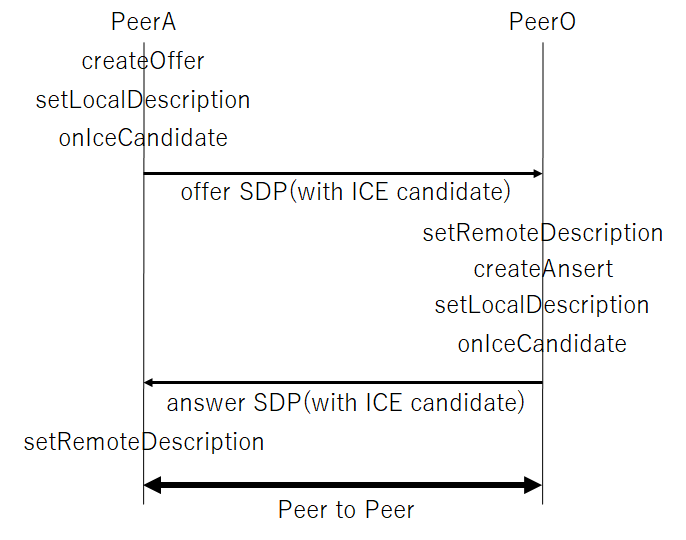
\includegraphics[width=10cm]{./assets/image/signaling.png}
	\caption{シグナリング}
	\label{fig:signaling}
\end{figure}
PeerAがcreateOfferを行いoffer側のSDPの作成準備を行う.
次にsetLocalDescriptionでSDPを作成し,
ICE candidateのリストアップを行う.
ICE candidateのリストアップが完了すると,
ICE candidateをoffer側のSDPの中に含ませて,PeerOへ送る.
PeerOはPeerAのoffer側のSDPをsetRemoteDescriptionで受け取り,
createAnswerでanswer側のSDPの作成準備を行う.
setLocalDescriptionでSDPを作成し,ICE candidateのリストアップを行う.
ICE candidateのリストアップが完了するとICE candidateを
answer側のSDPの中に含ませて,PeerAへ送る.
PeerAはPeerOのanswer側のSDPをsetRemoteDescriptionで受け取りP2P接続が完了する.

% ---------------------------------------------------------------------

\chapter{提案手法}
\section{概要}
本章では、Kademliaをベースに効率的にストリーム形式のデータを共有できる
システムであるLayeredKadを提案する。

Kademliaはデータを共有する際に、
そのデータをアルゴリズムに従いネットワーク全体に確率的に分散させる。
そのためKademliaで連続的なストリーム形式のデータを共有する場合、
個々のストリームのチャンクデータをネットワーク全体に対し
問い合わせを行い、処理する必要がある。
ライブ映像のようなチャンクの生成周期が非常に短く、
高頻度にデータ共有する必要がある場合、Kademliaでは、
ネットワーク全体に対して連続的にその都度、負荷をかけることになり、
データ共有の効率が非常に悪化することが予測される。

そこでLayeredKadでは共有するデータごとに別のKademliaネットワークを作成し
ネットワーク自体のスコープをデータごとに区切ることで、
ストリームデータのような連続的なデータでも効率よく共有できるようにする。

本手法では、共有するデータの情報をメタファイルに保存し、
Kademliaネットワーク上で共有する。
このメタファイルを共有するネットワークを
メインネットワークと定義する。
メインネットワーク上でメタファイルを所有するユーザ同士で
さらに別のKademliaネットワークを構築し、メタファイルの情報に従い
メタデータに対応する実体データの共有を行う。
この実体データを共有するネットワークをサブネットワークとする。
メインネットワークとサブネットワークの関係を図\ref{fig:image}
に示す。

\begin{figure}[H]
	\centering
	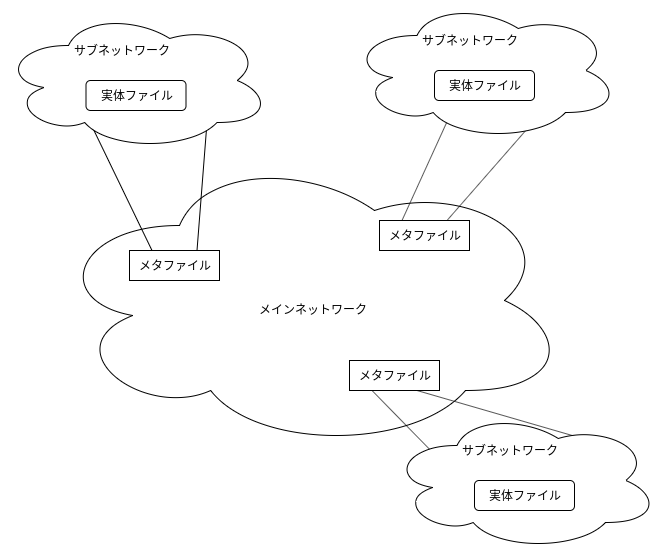
\includegraphics[width=10cm]{./assets/image/image.png}
	\caption{メインネットワークとサブネットワーク}
	\label{fig:image}
\end{figure}

\section{メタデータ}
LayeredKadでは静的、動的の両方のデータ形式の
共有に対応するためにメタデータとして
共有するデータの情報の共有を行う。
メタデータの基本構造は次のようになっている。
\begin{lstlisting}
type Meta = {
  type: "static" | "stream";
  name: string;
  payload: { [key: string]: any };
};
\end{lstlisting}

typeはメタデータの種類を表す。
本論文ではstaticとstreamの二種類が存在する。

nameはメタデータの名前である。nameには任意の文字列を与える。

payloadには実体データに関する情報を与える。

\subsection{StaticMeta}
静的なデータを扱うメタデータ
\begin{lstlisting}
type StaticMeta = Meta & {
  type: "static";
  payload: { keys: string[] };
};
\end{lstlisting}

payloadのkeysが実体データのハッシュキーの集合である。

\subsection{StreamMeta}
ストリーム(ライブ映像など)を扱うメタデータ
\begin{lstlisting}
type StreamMetaPayload = {
  first: string;
  width?: number;
  height?: number;
  cycle: number;
};	
type StreamMeta = Meta & {
  type: "stream";
  payload: StreamMetaPayload;
};  
\end{lstlisting}

payloadのfirstが実体データのストリームデータの
最初のチャンクのハッシュキーである。

width,heightは動画の縦横のピクセル数である。

cycleには "$ 1000 \div フレームレート $" の値を与える.

\subsubsection{ストリームデータ}
ストリームデータは複数の動的に生成される
チャンクデータから成り立つ。
本論文では一つのキー(最初のチャンクのハッシュキー)
から全チャンクデータを探索できるようにする必要がある。
そのため、チャンクデータをKademlia上に保存する際には、
そのチャンクデータ(便宜上chunksとする)の次に生成される
チャンクデータ(便宜上next chunksとする)が生成されるのを待ち、
chunksとnext chunksのハッシュキーを一つのvalueとして
にKademlia上に保存し、
next chunksのハッシュキーを辿ることで、ストリームデータ
を動的に継続的に取得できるようにしている。


\section{Network}
LayeredKadではネットワークがMainNetとSubNetの2階層存在する。

\subsection{MainNet}
Kademliaをベースとしたネットワークである。
ここでメタデータのやり取りと、新規参加ノードとSubNetとの橋渡しを行う。
MainNetにはStore,FindValue,DeleteValueの3つの命令が存在する。

\subsubsection{Store}

StoreはMainNet上にメタデータを保存する命令である。

Storeの型定義を以下に示す。
\begin{lstlisting}
	type Store = (meta: Meta) => 
		Promise<{ url: string, peers: Peer[] }>
\end{lstlisting}

Storeはメタデータを引数として実行する。
実行結果としてメタデータが保存されたアドレス(url)と
メタデータを受け取ったノードらの情報(peers)を返す。

\subsubsection{FindValue}

FindValueはurlに対応するメタデータを探す命令である。

FindValueの型定義を以下に示す。
\begin{lstlisting}
	type Store = (url: string) => 
		Promise<{ meta: Meta, peer: Peer }>
\end{lstlisting}

FindValueはurl文字列を引数として実行する。
実行結果としてメタデータ(meta)と、
そのメタデータを返却してきたノードの情報(peer)を返す。

\subsubsection{DeleteData}

DeleteDataは自身の持つメタデータを削除する命令である。

DeleteDataの型定義を以下に示す。
\begin{lstlisting}
	type Store = (url: string) => void		
\end{lstlisting}

DeleteDataはurl文字列を引数として実行する.

\subsection{SubNet}
Kademliaをベースとしたネットワークである。
メタデータの指し示すデータのやり取りを行う。
構造としては、一つのMainNet上に複数のSubNetが存在することになる。

\subsubsection{FindStaticMetaTarget}
静的なデータを扱うメタデータの実体データを探索する命令である。
型定義を以下に示す。
\begin{lstlisting}
	type FindStaticMetaTarget = () => Promise<ArrayBuffer | undefined>
\end{lstlisting}

SubNetの持つメタデータを元に実体データを探索し、
探索結果を返却する。

\subsubsection{FindStreamMetaTarget}
StreamMetaの実体データを探索する命令である。
型定義を以下に示す。
\begin{lstlisting}
	type FindStaticMetaTarget = (
		cb: (res: {
      			type: "error" | "chunk" | "complete";
      			chunk?: ArrayBuffer;
    			}) => void
		) => void
\end{lstlisting}
ストリームデータは長さが不明なので終了を持ち受けるのではなく、
入手したチャンクを都度コールバックで返却する。

\section{Actor}
ActorはMainNetとSubNetを利用し、
LayeredKadのシステムを実現するためのノードの実装である。
本論文ではSeeder,User,Navigatorの3つのActorが存在する。
一つのノードは同時に複数のActorになりうる。

\subsection{Seeder}
Seederとはメタデータの実体データを持つノードのことである。
Seederの中でも特に任意のデータをもとにメタデータを作成し、
メタデータをMainNet上にStoreし、SubNetを生成するSeederを
OriginSeederと定義するが、振る舞いは通常のSeederと変わらない。
SeederによってMainNet上でメタデータをStoreされたノードはNavigatorとなり、
SubNetへの接続を要求するUserとSeederの橋渡しを担う。
また、SeederもNavigatorとして振る舞う。

\subsubsection{SubNetの生成}
OriginSeederはメタデータをMainNetにStoreし、その結果
メタデータのurlとStore先のノード情報(peers)を得る。
OriginSeederはメタデータの情報を持ったSubNetを生成する。
そしてpeersの対象のノードたちをNavigatorにする。

\subsubsection{Seederの命令}
SeederにはOriginSeeder用の2種類の命令が定義されている。
\begin{itemize}
	\item{StoreStatic} \\
	静的なデータからメタデータを生成しMainNetに保存する。
	その後メタデータに対応するSubNetを生成し、
	メタデータの実体データをSubNetに保存する。
	
	型定義を以下に示す。
	\begin{lstlisting}
	type StoreStatic = (name: string, ab: Buffer) =>
		Promise<{url: string, meta: Meta}>
	\end{lstlisting}
	
	引数にメタデータの名前となる文字列と静的なデータを受け取る。
	メタデータのurlとメタデータを返却する。

	\item {StoreStream}\\
	ストリームデータからメタデータを生成しMainNetに保存する。
	その後メタデータに対応するSubNetを生成し、
	メタデータの実体データをSubNetに保存する。

	型定義を以下に示す。
	\begin{lstlisting}
	type StoreStream = (name: string, first: Buffer,
		payload:{width:number,heigh:number,cycle:number}
			) =>
		Promise<{event:Trigger,url:string}>
	\end{lstlisting}

	引数にメタデータの名前となる文字列と
	ストリームデータの最初のチャンクデータと
	ストリームデータの情報を受け取る。
	戻り値のTriggerはfirstチャンク以降のチャンクデータを送るための
	コンポーネントである。urlはメタデータのurlである。
\end{itemize}

\subsection{User}
UserはメタデータのURLをもとにMainNet上でメタデータを探索し、
メタデータに対応するSubNetと接続する。
メタデータを持つNavigatorを仲介としてSeederと接続する。
SeederとUserのピアはSubNet上で管理される。
SubNetと接続しているUserを特にObserverと呼ぶ

\subsubsection{Userの命令}
Seederには1種類の命令が定義されている。
\begin{itemize}
	\item {ConnectSubNet}\\
	urlを元にMainNet上でメタデータを探索し、メタデータを
	与えてくれたノードをNavigatorとしてメタデータの実体データを
	持つ、SeederのSubNetへ接続する。\\

	型定義を以下に示す。
	\begin{lstlisting}
	type ConnectSubNet = (url: string) =>
		Promise<{subNet: SubNet,meta:Meta}>
	\end{lstlisting}

	メタデータのurlを受け取り、
	SubNetとメタデータを返却する。		
\end{itemize}

UserはConnectSubNetによって接続したSubNetに対して
FindStaticMetaTargetやFindStreamMetaTargetを行うことによって
メタデータの実体データを探索し入手する。

\subsection{Navigator}
NavigatorはUserをMainNetとSubNet間の橋渡しを行うActorである。
MainNetを監視しており、UserからConnectSubNet命令を受け取った時に、
Navigatorと接続されたSeederとUserの接続を仲介する。

\subsubsection{Seederとの接続}
LayeredKadのノードはメタデータをStoreされると、Navigatorとなるので、
すべてのノードが潜在的にNavigatorになるうる。
そこで、これからNavigatorになるノードのことをNavigatorCandidateと定義する。
NavigatorCandidateはMainNetを監視しており、
自らにメタデータをStoreされた時に、Storeしてきたノード(Seeder)に
対してpeerを生成しコネクションを維持する。
これによりNavigatorCandidateはNavigatorとなる。

\subsubsection{UserとSeederの接続仲介}
NavigatorはMainNetを監視し、
Userが自らの持つメタデータを探索によって発見し、SubNetへの接続要求である。
ConnectSubNet命令を実行した際に自らの接続するSeederに対してUserとの
接続を行うための情報を要求する(WebRTCのSDP等)その情報をUserへ返却し、
次にUserの接続情報(SDP等)をSeederへ渡す。
これによりUserとSeederの間にpeerが生成され接続が完了する。
SeederはSubNet環境下に存在するので、
Userはメタデータに対応するSubNetに接続できたことになる。


\section{実装}
TypeScriptを用いてNode.jsとChrome上で動作するように実装を行った。
P2P通信部部にはWebRTCを用いている。

通常のKademliaと本手法のLayeredKadの性能比較を行うために、
Node.js上で動作するベンチマーカーの実装を行った。
なお、ベンチマーカーは実装の都合上P2P通信部分はWebRTCではなく、
UDPを使用している。

% ---------------------------------------------------------------------
\chapter{評価実験}
\section{仮説}
本論文では、データ通信量と、タスクの処理時間の2つの観点から、
LayeredKadの評価を行う。
現実的なユースケースを想定し、
幾つかのファイルがネットワーク上に共有され、
それぞれのファイルに関心があるユーザがそれぞれのグループを形成して
共有しあっているケースを想定し仮説を立てる。
\subsection{データ通信量}
LayeredKadでは共有するデータごとにネットワークを分割しており、
データの保存や探索がネットワーク全体に影響しないので、
Kademliaとノード数が同じであれば、ネットワーク全体における、
データ通信量が少なくなることが予想される。
ファイル共有サービスにおいてファイル共有速度の最も大きな
ボトルネックはネットワークの通信速度であるので、
データ通信量が少ないことはメリットである。
\subsection{タスクの処理時間}
LayeredKadはKademliaをさらに構造化したシステムであるため、
単純に一つのファイルを共有するようなケースでは、
当然、Kademliaの方が高速である。
しかし、今回のケースではKademliaはすべてのファイルについての
処理においてもネットワーク全体で処理を行う必要があるのに対して、
LayeredKadではユーザグループ(SubNet)内で完結するため、
処理効率がよく、タスクの処理時間も短くなると考えられる。

\section{結果}
\subsection{データ通信量}
\subsubsection{実験}
データ通信量の計測を行うために、KademliaとLayeredKadで
データ通信量の計測を行うベンチマークプログラムを作成した。
ベンチマークプログラムは表\ref{table:spec-note}の環境で実行した。

\begin{table}[H]
	\caption{スペック}	
	\centering
	\label{table:spec-note}
	\begin{tabular}{|l|l|}
		\hline
		CPU &   
		Intel Core i7-7500U 2.70GHz 2Core 4Threads\\ 
		\hline	
		OS  &   
		Ubuntu 19.10 \\ 
		\hline
	\end{tabular}	
\end{table}

本ベンチマークプログラムでは、ノードのペアを1グループとして、
ファイル共有を行わせる。
ベンチマークプログラムのシナリオのイメージを
図\ref{fig:trafficBenchmark}に示す

\begin{figure}[H]
	\centering
	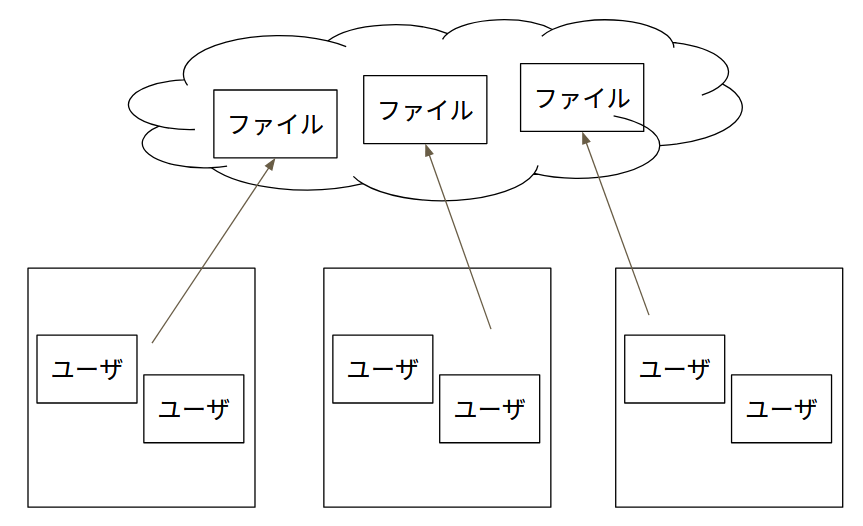
\includegraphics[width=10cm]{./assets/image/traffic_benchmark.png}
	\caption{通信量ベンチマークのイメージ}
	\label{fig:trafficBenchmark}
\end{figure}

ノード数を変数パラメータとして、パラメータを増加させて
LayeredKadとKademliaのデータ通信回数を記録し、比較を行う。

\subsubsection{実験結果}

\begin{table}[H]
	\caption{実験結果}	
	\centering
	\label{table:traffic-result}
	\begin{tabular}{|l|l|l|}
		\hline
		ノード数     &   
		Layered Kad(回) &   
		Kademlia (回)\\ 
		\hline
		10               &   
		10               &   
		380\\
		\hline
		30               &   
		16               &   
		729\\
		\hline
		40               &   
		32               &   
		1026\\
		\hline
		50               &   
		33               &   
		1278\\
		\hline
	\end{tabular}	
\end{table}

\begin{figure}[H]
	\centering
	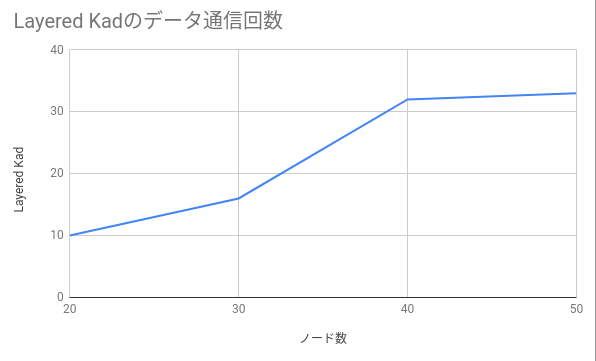
\includegraphics[width=10cm]{./assets/image/layered-kad_traffic.png}
	\caption{layeredKadの通信量}	
\end{figure}

\begin{figure}[H]
	\centering
	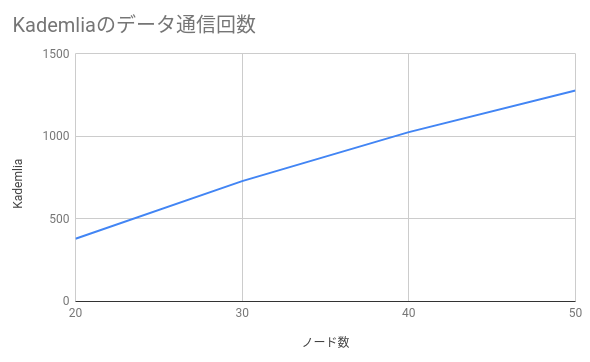
\includegraphics[width=10cm]{./assets/image/kad_traffic.png}
	\caption{kademliaの通信量}	
\end{figure}

\begin{figure}[H]
	\centering
	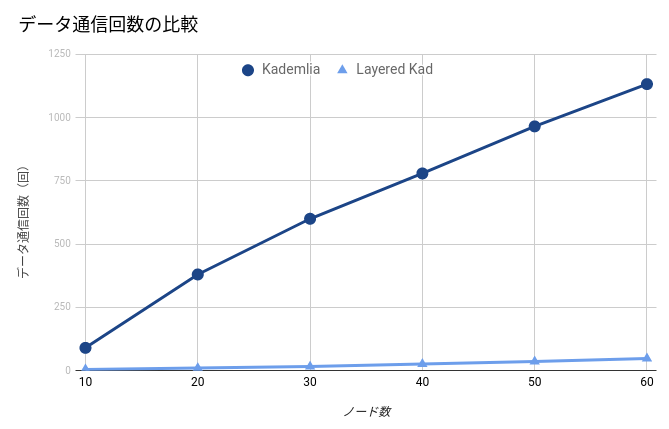
\includegraphics[width=10cm]{./assets/image/traffic_graph.png}
	\caption{通信量の比較}
	\label{fig:traffic-graph}
\end{figure}

\subsection{タスク処理時間}
\subsubsection{実験}
タスク処理時間の計測を行うために、KademliaとLayeredKadで
タスク処理時間の計測を行うベンチマークプログラムを作成した。
ベンチマークプログラムは表\ref{table:spec-ryzen}の環境で実行した。

\begin{table}[H]
	\caption{スペック}	
	\centering
	\label{table:spec-ryzen}
	\begin{tabular}{|l|l|}
		\hline
		CPU &   
		Ryzen Threadripper 2950X 3.50Ghz 16Core 32Threads \\ 
		\hline	
		OS  &   
		Ubuntu 18.04 \\ 
		\hline
	\end{tabular}	
\end{table}

ベンチマークプログラムのシナリオはデータ通信量のベンチマーカーと
同じであるが、タスク処理時間をより正確に計測するために、
1ノードに付き、CPUのスレッド1つを割り当てるようにベンチマークプログラムの
マルチスレッド化を行っている。本実験では、ノード数は16ノードで固定とし、
共有するデータ数のチャンキング数を変数として実験を行う。

\subsubsection{実験結果}
\begin{table}[H]
	\caption{実験結果}	
	\centering
	\label{table:calc-result}
	\begin{tabular}{|l|l|l|}
		\hline
		チャンク数 &   
		Layered Kad (s) &   
		Kademlia (s)\\ 
		\hline
		1               &   
		2.098           &   
		0.636\\
		\hline
		4               &   
		2.728           &   
		2.032\\
		\hline
		5               &   
		2.469           &   
		2.435\\
		\hline
		6               &   
		2.581           &   
		2.679\\
		\hline
	\end{tabular}	
\end{table}

\begin{figure}[H]
	\centering
	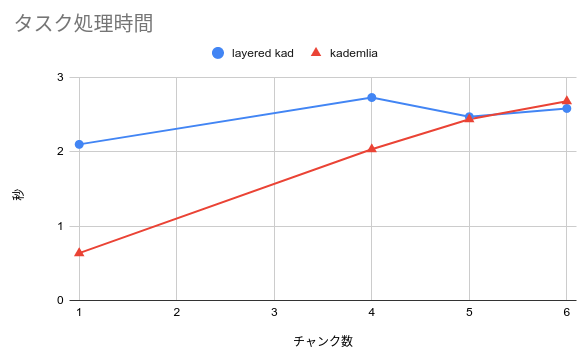
\includegraphics[width=10cm]{./assets/image/calc_compare.png}
	\caption{タスク処理時間の比較}
	\label{fig:calc_compare.png}
\end{figure}

\section{考察}
\subsection{データ通信量}
実験結果は、仮説の通りの結果となった。
ただし、この結果はベンチマークのシナリオが
LayeredKadが共有するデータ毎に別のネットワークを構築するという性質に
有利な設定であるため、これほどの性能差が出たと考えられる。

\subsection{タスク処理時間}
LayeredKadではデータのチャンキング数が増加しても
タスク処理時間は概ね変化しないのに対して、
Kademliaではチャンキング数の増加に対してタスク処理時間が比例増大
していることがわかる。
LayeredKadでは、いくらチャンク数が増えたとしてもサブネットワークのペアとなるノードとの
一対一の通信回数がチャンク数分増えるだけなのに対して、
Kademliaはチャンク数分、ネットワーク全体に対して問い合わせるため、
その分処理時間が増大していると考えられる。

% ---------------------------------------------------------------------

\chapter{おわりに}
\section{結論}
本論文では、Kademliaをベースに効率的に静的なデータやストリーム形式の
データを共有できるシステムの開発を行った。
ネットワークを共有するデータ毎に分割し、非効率的なデータ通信を削減する
ための仕組みであるLayeredKadを考案し、実装した。
静的なデータや動的なデータなどを柔軟に扱えるようにするために、メタデータ
を共有する仕組みを考案した。
メタデータを共有するネットワークをメインネットワークとし、
メタデータの実体データを共有するネットワークをサブネットワークとし、
ネットワークの分割を実現した。

LayeredKadの性能を評価するため、ユーザが実利用する際のシチュエーション
に沿ったシナリオ上で、LayeredKadとKademliaのベンチマークを行い
性能の評価を行った。
ベンチマークはネットワークのボトルネックとなるデータ通信と、
タスク処理時間の二項目に着目して行った。
データ通信のベンチマークでは、LayeredKadはそのネットワーク分割能力
によってKademliaよりデータ通信量が小さいごとを実証できた。
タスク処理時間のベンチマークでは、Kademliaがチャンク数の増加に対して
処理時間が比例増大したのに対して、
LayeredKadではチャンク数の増加が処理時間に影響しないことがわかった。

\section{課題}
Kademliaはネットワーク全体に一定のルールでデータを保存しているが、
LayeredKadでは実体のデータはデータを利用するユーザ間でのみデータが
保存されている。そのためデータの冗長性という面ではKademliaに劣っている。
また、Kademliaは様々なサービスに応用され長期間の安定した動作が
確認されているが、本論文ではLayeredKadの長期間の安定動作については
検証しておらず、未知の問題が存在する可能性がある。

\begin{acknowledgment}
	本研究を進めるにあたり, ご指導を頂いた指導教員の萩原助教授に感謝致します.
	日頃の議論において助言や知識を頂いた萩原研究室の皆様に感謝します.
\end{acknowledgment}

\bibliographystyle{unsrt}
\bibliography{reference}
\end{document}